%
\chapter{Distributed evaluation of monitoring goals}
%


\section{Distributed runtime model}

As it has been stated before, the model of the system is stored distributedly on different computation units. A model element is only stored on a given computation unit. References can occur between elements in different partitions, so we create proxy objects, that represents an object from another partition, and the local object stores reference to proxy object. For example, on figure~\ref{fig:distrib-model-example} this can be seen. There are 4 segments, \texttt{S1},\texttt{S2}, \texttt{S3}, \texttt{S4} and two trains, \texttt{T5} and \texttt{T6}. If we allocate \texttt{S1}, \texttt{S2}, \texttt{T5} to one computation unit, and \texttt{S3}, \texttt{S4}, \texttt{T6} to another, we must deal with the edges between \texttt{S2} and \texttt{S3} We solve this by creating a proxy objects refering to their corresponding remote nodes and refer to them instead of the original, unavailable node.

\begin{figure}[h]
	\begin{center}
		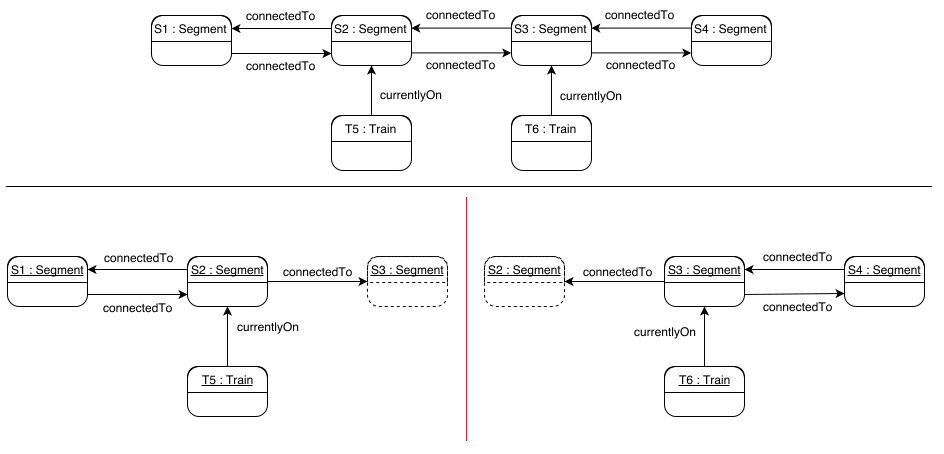
\includegraphics[width=\textwidth]{figures/distributed-model.png}
		\caption{Example for edges between nodes}
		\label{fig:distrib-model-example}
	\end{center}
\end{figure}




\section{Distributed query execution}


\subsection{Distributed local search-based pattern matching}

As models are stored on different computational units we still needs to find matches, that can span over multiple model parts. To find matches for a pattern local search algorithm is used in a distributed way. Search operations are being executed locally, and if the next operation needs to be executed on multiple nodes, the search context, (ie.\ the bound variables and the operations number) are sent to other computational units.

\begin{figure}[h]
	\begin{center}
		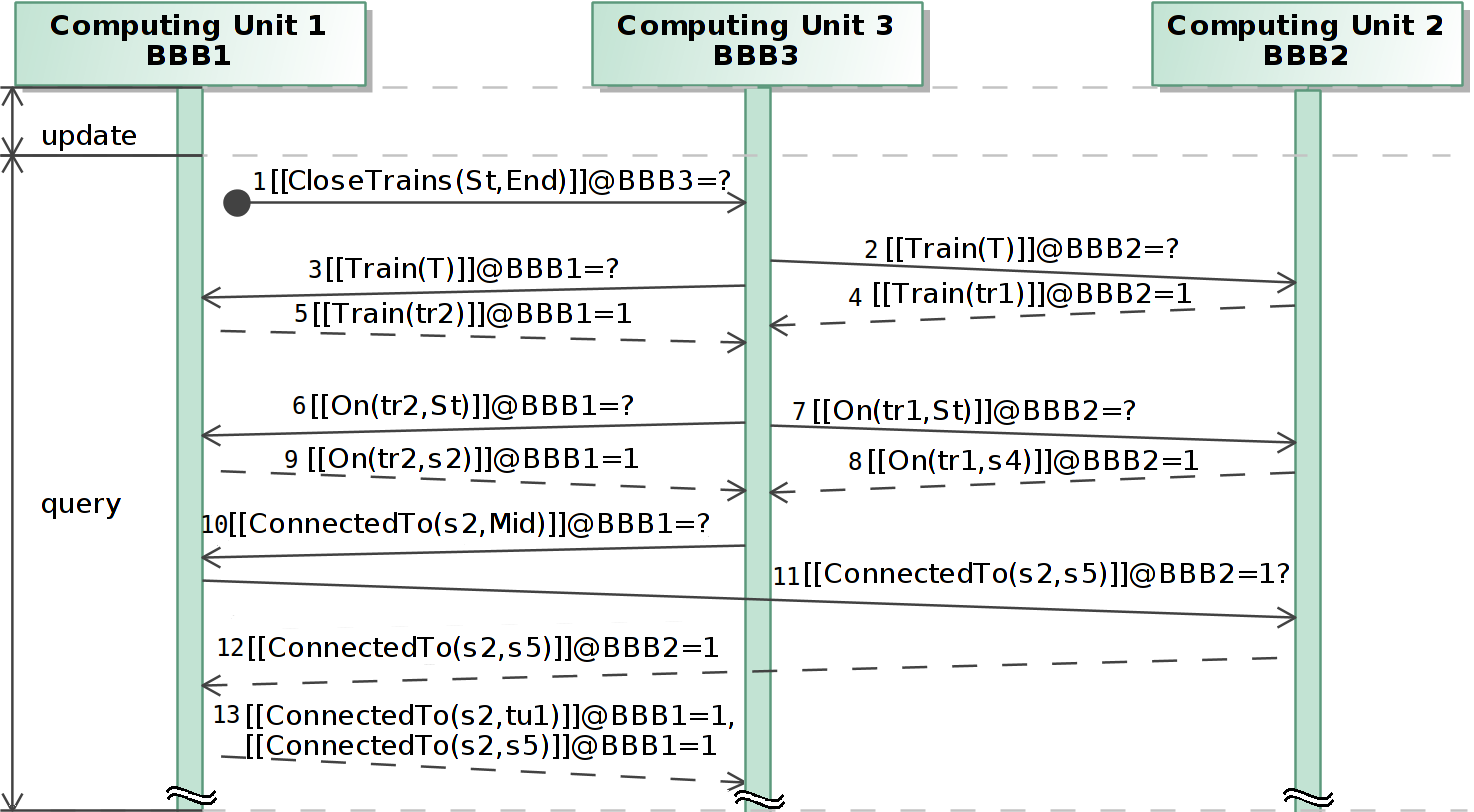
\includegraphics[width=1\textwidth]{figures/seq-diagram-query-exec.png}
		\caption{Sequence diagram of an example query execution}
		\label{fig:distibuted-exec}
		
	\end{center}
\end{figure}



